% ---------------------------------------------------------------------------
% Supplementary material for
%   "How Fast Does Taste Go Stale? Measuring Data Aging in Recommenders,
%    and When You Cannot"
% Technical appendix accompanying the WSDM 2027 paper
% (https://doi.org/10.1145/3862322.3863817).
% ---------------------------------------------------------------------------
\documentclass[10pt,letterpaper]{article}

\usepackage[margin=1in]{geometry}
\usepackage{booktabs}
\usepackage{amsmath,amssymb}
\usepackage{graphicx}
\usepackage{caption}
\usepackage[hidelinks]{hyperref}
\usepackage{url}
\usepackage{microtype}

\newcommand{\Tdrift}{T_{\mathrm{drift}}}
\newcommand{\ecov}{e_{\mathrm{cov}}}

% S-numbering for sections, tables and figures
\renewcommand{\thesection}{S\arabic{section}}
\renewcommand{\thetable}{S\arabic{table}}
\renewcommand{\thefigure}{S\arabic{figure}}
\renewcommand{\theequation}{S\arabic{equation}}
\makeatletter
\patchcmd{\l@section}{1.5em}{2.3em}{}{}
\makeatother

\title{\vspace{-1.5em}Supplementary Material\\[0.3em]
\large How Fast Does Taste Go Stale?\\
Measuring Data Aging in Recommenders, and When You Cannot}
\author{\normalsize Minghao Chen$^{1}$, Wentao Mo$^{1}$, Jiali Wang$^{1}$, Xun Zhang$^{1}$, Zhenfeng Liang$^{1}$, Yi Zeng$^{1}$, and Jiale Zheng$^{2,\ast}$\\[0.3em]
\small $^{1}$Tencent, Shenzhen, China \qquad $^{2}$Huawei, Shenzhen, China\\[0.15em]
\small $^{\ast}$Corresponding author: \texttt{zhengjiale2@huawei.com}}
\date{}

\begin{document}
\maketitle
\vspace{-1.5em}

\noindent
This technical appendix accompanies our WSDM 2027 paper
(\href{https://doi.org/10.1145/3862322.3863817}{doi:10.1145/3862322.3863817})
and presents the complete per-domain tables across all 23 domains, extended
derivations, and protocol sensitivity analyses.

\tableofcontents
\bigskip

% ===========================================================================
\section{Protocol, fitting procedure, and quality control}
\label{sup:protocol}

\paragraph{Units and effect sizes.}
Throughout the paper and this supplement, $1$\,mnat $= 10^{-3}$ nats of test
loss, and all slopes are reported per $e$-fold of training-window age. The
age effect is small in absolute terms: over the full probed range, overall
loss moves by $7$--$130$\,mnat, with a median of $19$\,mnat across the 23
domains ($7.1$ on KuaiRand, $29$ on MovieLens, and $130$ on KuaiRec).
Signal-to-noise ratios of $20$--$70\times$ relative to seed variance confirm
that these trends are genuine, but practical significance should be judged on
the ranking metric rather than the loss exponent: across the backtest's
$22\times$ cadence range, volume-weighted serving loss moves by only
$4.2$\,mnat whereas serving AUC drops by $1.9$ points ($0.6207 \to 0.6022$).

\paragraph{Probe and budget.}
Every measurement in the study uses a biased matrix-factorization probe,
$\hat y = \mu + b_u + b_i + p_u^\top q_i$ with $d = 32$ latent dimensions
unless stated otherwise, trained with binary cross-entropy on logits,
sparse--dense Adam (sparse gradients for the embedding tables, dense for the
scalars), batch size $8{,}192$, learning rate $3\times10^{-3}$, and at most
$8{,}000$ optimizer steps. We report test loss at the best early-stopping
checkpoint within that budget, selected directly on the evaluation set without a
separate validation split (Section~\ref{sup:valstop} quantifies the resulting
optimism). Any run whose loss remains above the $\ln 2$ chance threshold is
flagged as diverged and retuned rather than reported.

\paragraph{Windows, subsampling, and seeds.}
Any candidate training window with fewer than $25{,}000$ events is dropped
(and logged); all surviving windows within a domain are uniformly subsampled to
the smallest surviving volume, capped at $300{,}000$ events. By default, each
age cell uses three model seeds. Table~6 of the main paper uses nine model seeds
for its primary curves (plus a matched nine-seed redraw on Game-UGC;
\S\ref{sup:cohorts}), except for the eight Amazon item cohorts, which retain
three. Increasing from three to nine seeds narrowed MovieLens's
$\mathrm{u}{\cap}\mathrm{i}$ interval from $[1{,}032, 3{,}355]$ to
$[1{,}031, 1{,}768]$\,d, moved Netflix's item cohort from $927$ to $888$\,d,
kept Game-UGC draw~0 at $4.63{\to}4.60$\,d, and shifted BeerAdvocate's
truncation spread across the $1.5\times$ cutoff ($1.46\times{\to}1.87\times$).

Cohort runs fix the subsample seed so that the training subsample is
bit-identical across model seeds and cohort membership is well defined; these
runs use only the translated~(A) arm.

\paragraph{Fitting.}
For a fixed $\delta$, the Box--Cox law
\begin{equation}
L_X(\tau) = c_X + \beta \cdot \frac{(\tau/\tau_0)^{\delta}-1}{\delta},
\qquad X \in \{A, B\}
\label{eq:boxcox}
\end{equation}
is linear in the two intercepts $c_A, c_B$ and in $\beta$, so we find
$\delta$ by a global grid scan and solve the linear part exactly at each
grid point subject to $\beta \ge 0$. The objective is unweighted least
squares on the per-cell means, so three-seed and nine-seed cells receive
equal weight despite unequal variance. Ninety-percent confidence intervals come
from a 300-draw percentile bootstrap over runs within each cell; at three seeds
per cell, this resamples from only ten distinct multisets and is
correspondingly coarse. Both choices reinforce the main paper's caveat that
seed-only intervals represent lower bounds on total uncertainty.

\paragraph{Flags and pre-stated quality control.}
A fit landing within $10^{-3}$ of a $\delta$ boundary is flagged
\emph{at bound} and refit over the wider parameter bounds $\delta \in [-6, 4]$;
a curve that would need $\beta < 0$ is flagged \emph{descending} rather than
forced to zero. Our pre-stated quality-control rule flags any fit with
$\beta < 10^{-6}$ or $R^2 < 0.2$ as ``no measurable drift'' (8 of the 68 fits).

Because $R^2$ is computed against the global mean while Eq.~\eqref{eq:boxcox}
fits a separate intercept per arm, an arm-level offset alone inflates $R^2$. When
scored instead against the two-intercept $\beta = 0$ null (which isolates the
age term), exactly one fit in the panel changes its verdict: Amazon Musical
Instruments drops from $R^2 = 0.25$ to $0.01$. Because this category sets the
lower endpoint of the measured exponent range, the main paper reports that range
both with it ($[-3.2, 2.2]$) and without it ($[-1.9, 2.2]$, bounded below by
the game-UGC finish label).

\paragraph{The model-free timescale $\tau_{1/2}$.}
The half-rise time $\tau_{1/2}$ interpolates in log-age between the \emph{first}
pair of cells bracketing half of the cohort loss increase observed at the
oldest probed age, accompanied by a 200-draw bootstrap; on a non-monotone curve,
taking the first crossing yields the more conservative (earlier) estimate.
Degenerate cells and noise-level curves are excluded under pre-stated rules.
An estimate $\tau_{1/2}$ is classified as \emph{truncation-stable} when its
refits across truncation horizons span a factor of less than $1.5$.

\paragraph{Hill fits.}
We attempt Hill fits only on curves passing four pre-stated gates
($\Tdrift \in [\tau_{\min}/2,\, 2\tau_{\max}]$, interior $\theta$, observed
deceleration, and $A > 0$); 6 of the 33 cohort curves qualify. We do not
adjudicate between shared and per-domain Hill shapes---not because the two tie,
but because both models are severely overparameterized at $k \approx n/2$:
although AIC favors the shared shape ($\Delta\mathrm{AIC} = -56$ at
$k = 100$--$132$, $n = 221$) and $\mathrm{AICc}$ favors it even more strongly
($\Delta\mathrm{AICc} \approx -287$), residual-based model selection is
uninformative in this regime.

\paragraph{Run accounting.}
The baseline GPU sweep comprises $5{,}296$ training runs (roughly 40 GPU hours
on a single NVIDIA GTX~1660, 6\,GB; any single domain reproduces in about an hour),
tallied by \texttt{src/paper\_numbers.py} under a stated inclusion rule:
$2{,}229$ runs across the 68 baseline measurement settings, $1{,}728$ in the
test-period sweep, $526$ in the initial backtest and policy variants
(including two warm-start configurations superseded during tuning), $777$
in convention-sensitivity reruns (held-out stopping rule, second
cohort draw, volume-matched backtest, and recency half-life sweep), and $36$ in
weekday controls, excluding $98$ early exploratory runs. An extended CPU
diagnostic suite (\texttt{SparseAdam}) adds $1{,}385$ runs, bringing the study
census to $6{,}681$:
$522$ for the 23-domain four-way warm/cold partition (\S\ref{sup:derivations}),
$296$ for three strictly non-overlapping rolling backtests (\S\ref{sup:backtest}),
$114$ for three-domain static side-feature controls (\S\ref{sup:invariance}), and
$453$ for game-UGC multi-draw, validation-stopping, and 1-day grid checks
(\S\ref{sup:cohorts}).

% ===========================================================================
\section{Derivations}
\label{sup:derivations}

\subsection{The Box--Cox family and its logarithmic interior point}

Write $g_\delta(x) = (x^{\delta} - 1)/\delta$ for $x > 0$. For
$\delta \neq 0$ this is the Box--Cox transform; its limit as
$\delta \to 0$ is
\[
\lim_{\delta \to 0} \frac{x^{\delta} - 1}{\delta}
= \lim_{\delta \to 0} \frac{e^{\delta \ln x} - 1}{\delta}
= \ln x ,
\]
uniformly on compact subsets of $(0, \infty)$. Substituting
$x = \tau/\tau_0$ into Eq.~\eqref{eq:boxcox} therefore gives
$L_X(\tau) \to c_X + \beta \ln(\tau/\tau_0)$: the logarithmic age law is an
\emph{interior} point of the family rather than a degenerate corner, and
$\delta$ is a continuous ``drift shape'' coordinate. Values $\delta > 0$
correspond to accelerating decay (loss grows faster than logarithmically with
age), whereas $\delta = 0$ recovers logarithmic growth; for every $\delta < 0$,
loss approaches the finite asymptote $c_X - \beta/\delta$ as age grows. The
boundary at $-1$ concerns integrability at zero age in the serving-time average
below, not boundedness at large age.

The parameterization is also scale-anchored: $g_\delta(1) = 0$ for every
$\delta$, so $c_X = L_X(\tau_0)$ regardless of $\delta$, and the two arms'
intercepts are directly comparable across fits with different exponents.

\paragraph{The single modeling assumption behind a shared $(\beta,\delta)$.}
Summarizing an entire window by a single age $\tau$ introduces an aggregation
approximation: for a nonlinear transform $g$, the average of $g$ across
individual event ages generally differs from $g$ evaluated at the mean age, by
an amount governed by $g$'s curvature and the within-window age distribution.
Consequently, the widened~(B) arm is especially sensitive to the
calendar-midpoint convention (\S\ref{sup:agewt}).

\subsection{Serving-time average of the age law}

Absorb the Box--Cox normalization into a power form,
\[
L(\tau) = L_0 + b\,\tau^{\delta}, \qquad
b = \frac{\beta}{\delta\,\tau_0^{\delta}}, \qquad
L_0 = c - \frac{\beta}{\delta} .
\]
A model retrained every $P$ time units serves data whose age sweeps
$[0, P]$ uniformly in serving time, so the serving-time average loss is
\begin{equation}
\bar L(P) \;=\; \frac{1}{P}\int_0^{P} \! \big(L_0 + b\,\tau^{\delta}\big)\,
\mathrm{d}\tau
\;=\; L_0 + \frac{b}{\delta+1}\,P^{\delta},
\label{eq:lbar}
\end{equation}
which requires $\delta > -1$ for the integral to converge at $\tau \to 0^+$.

\subsection{The closed-form optimal period}

Add a retraining price $\lambda C / P$ per unit serving time, where $C$ is
the cost of one retrain and $\lambda$ converts it into loss units. The
objective is
\[
J(P) \;=\; L_0 + \frac{b}{\delta+1}P^{\delta} + \frac{\lambda C}{P},
\qquad
J'(P) \;=\; \frac{b\,\delta}{\delta+1}P^{\delta-1} - \frac{\lambda C}{P^{2}} .
\]
Setting $J'(P) = 0$ gives
\begin{equation}
P^{\ast} = \left[ \frac{\lambda C\,(\delta+1)}{b\,\delta}
\right]^{\frac{1}{1+\delta}} .
\label{eq:pstar}
\end{equation}

\paragraph{Validity for $-1 < \delta < 0$.}
For a saturating fit, $b = \beta/(\delta\tau_0^{\delta})$ is negative
(because $\beta \ge 0$ and $\delta < 0$), so the bracket in
Eq.~\eqref{eq:pstar} looks ill-defined at first sight. It is not: the
product
\[
b\,\delta \;=\; \frac{\beta}{\tau_0^{\delta}} \;=\; \beta\,\tau_0^{-\delta}
\;>\; 0 ,
\]
so the right-hand side of Eq.~\eqref{eq:pstar} is positive whenever
$\beta > 0$. The second derivative at that stationary point,
\[
J''(P) = \frac{b\,\delta(\delta-1)}{\delta+1}P^{\delta-2}
+ \frac{2\lambda C}{P^{3}},
\]
is positive there; moreover, $J(P) \to +\infty$ both as $P \to 0^{+}$ (where
the $-\lambda C / P^{2}$ term of $J'$ dominates $P^{\delta-1}$ for $\delta > -1$,
so $J' < 0$) and as $P \to \infty$ (where $J' > 0$), making the stationary
point the unique interior minimum. The economic content is that a saturating
domain has a \emph{bounded} staleness cost, not that the cadence trade-off
disappears.

\paragraph{The logarithmic limit.}
At $\delta=0$, $\bar L(P)=c+\beta[\ln(P/\tau_0)-1]$ and
$J'(P) = \beta/P - \lambda C/P^{2}$, so
$P^{\ast} = \lambda C / \beta$, which is the $\delta \to 0$ limit of
Eq.~\eqref{eq:pstar}. The closed form is therefore continuous across the
logarithmic case, matching the continuity that motivates the Box--Cox family
in the first place.

\paragraph{Where it fails.}
At $\delta \le -1$ the integral in Eq.~\eqref{eq:lbar} diverges at
$\tau \to 0^{+}$ and the serving average is undefined. This is an artifact
of extrapolating a fit made on $[\tau_0, \tau_{\max}]$ below $\tau_0$, not a
property of the cadence problem: no probe in this study is ever trained on
data younger than $\tau_0$.

\subsection{Two approximations in the main text}

\paragraph{Which coefficient enters $P^\ast$.}
Equation~\eqref{eq:pstar} is stated in terms of $b$, the coefficient of the
\emph{instantaneous} age law. Substituting the serving-average coefficient
$b/(\delta+1)$ instead would multiply $P^\ast$ by
$(\delta+1)^{1/(1+\delta)}$, or about $1.4\times$ at $\hat\delta \approx 1$
on the validation domain. Every number in the paper uses $b$ as defined
above.

\paragraph{Data are never fresh at the instant of retraining.}
As written, $\bar L(P)$ assumes zero data age at the instant of retraining,
whereas the freshest training window already has mean age $a \approx W/2$.
Retaining that base-age offset yields
\[
\bar L(P) = L_0 + \frac{1}{P}\int_{a}^{P+a} \! b\,\tau^{\delta}\,
\mathrm{d}\tau
= L_0 + b\,\frac{(P+a)^{\delta+1} - a^{\delta+1}}{(\delta+1)\,P} .
\]
Because $[a, P+a]$ stays bounded away from $\tau = 0$ for $a > 0$, this offset
serving average remains finite even when $\delta \le -1$ (where the $a = 0$
integral diverges at $\tau \to 0^+$), and accounting for $a > 0$ prevents
severe underestimation of $P^\ast$ when $\delta \le 0$ (\S\ref{sup:backtest}).
Integrating by parts rewrites the first-order condition for $\lambda C > 0$ as
$\int_0^{P^\ast} t L'(a+t)\,\mathrm{d}t = \lambda C$, whose left-hand side
increases monotonically with $P^\ast$ whenever $L$ is increasing. Since
$L'(x) = \beta\tau_0^{-\delta}x^{\delta-1}$ (including the $\delta \to 0$
limit), raising $a$ shortens $P^\ast$ for $\delta > 1$, leaves $P^\ast$
unchanged at $\delta = 1$ (where the offset adds only the constant $ba$ to
$\bar L$), and lengthens $P^\ast$ for $-1 < \delta < 1$. RecFlow's Arm-A fit
($\delta = 1.015$) sits near this neutral $\delta = 1$ boundary.

\subsection{The two-term identity}

Every run records the overall loss $L$, the warm-subset loss
$L_{\mathrm{warm}}$ (over test events whose user and item both appear in the
subsampled training window), and the warm coverage $\omega$ (the warm fraction
of test events). Because warm and cold partition the test set,
\begin{equation}
L \;=\; \omega \cdot L_{\mathrm{warm}} \;+\; (1 - \omega)\,L_{\mathrm{cold}},
\label{eq:twoterm}
\end{equation}
so $L_{\mathrm{cold}} = (L - \omega\,L_{\mathrm{warm}})/(1 - \omega)$ is
recoverable algebraically, without any additional fit, wherever
$\omega < 1$. Differentiating Eq.~\eqref{eq:twoterm} with respect to
$\ln\tau$ yields the continuous-age decomposition:
\[
\frac{\mathrm{d}L}{\mathrm{d}\ln\tau}
= \underbrace{\omega \frac{\mathrm{d}L_{\mathrm{warm}}}{\mathrm{d}\ln\tau}}
  _{\text{within warm traffic}}
+ \underbrace{(1-\omega)\frac{\mathrm{d}L_{\mathrm{cold}}}{\mathrm{d}\ln\tau}}
  _{\text{cold term}}
+ \underbrace{(L_{\mathrm{warm}} - L_{\mathrm{cold}})
  \frac{\mathrm{d}\omega}{\mathrm{d}\ln\tau}}_{\text{coverage collapse}} .
\]
When coverage falls and warm loss is lower than cold loss, the third term
is positive: transferring weight to the higher-loss group increases loss.
Its sign does not determine the curvature of the mixture.

For adjacent measured ages the same identity holds exactly in finite
differences, with each weight and each multiplying loss replaced by its
two-endpoint arithmetic mean. Within each age cell, we average $L$, $\omega$,
and $\omega L_{\mathrm{warm}}$ across seeds before recovering the conditional
losses from their probability masses. Summing adjacent finite differences
across ages yields three additive terms (in nats) that sum identically to total
aging $\Delta L$ (oldest minus freshest loss). We report percentage shares
across the 18 Arm-A domains that exhibit positive net aging ($\Delta L > 0$) and
pass the baseline apparent-drift screen; individual shares may be negative or
exceed $100\%$. Because this identity partitions observed test mixtures, the
three terms are descriptive rather than causal.

\paragraph{Four-way partition and internal cold-mix decomposition.}
To disaggregate the pooled cold subset, we reran all 23 domains on CPU while
logging the four disjoint subsets $g \in \{\mathbf{11}, \mathbf{10},
\mathbf{01}, \mathbf{00}\}$ (warm, user-seen/item-unseen, user-unseen/item-seen,
and mutually unseen; 522 runs, maximum mean-loss difference $0.003$ vs.\ the
baseline GPU sweep, and exact $\omega_{11} = \omega_{\mathrm{warm}}$ parity).
Writing $L = \sum_g \omega_g L_g$, the exact adjacent-age finite difference
generalizes Eq.~\eqref{eq:twoterm} to $\Delta L = \sum_g \bar\omega_g \Delta L_g +
\sum_g \bar L_g \Delta\omega_g$. Similarly, writing $\tilde\omega_g =
\omega_g / (1 - \omega_{11})$ for $g \in \{\mathbf{10}, \mathbf{01}, \mathbf{00}\}$
decomposes $\Delta L_{\mathrm{cold}}$ into within-group aging
$\sum_{g \neq 11} \bar{\tilde\omega}_g \Delta L_g$ plus internal cold-mix shift
$\sum_{g \neq 11} \bar L_g \Delta\tilde\omega_g$ (whose $\bar\omega_{\mathrm{cold}}$-weighted
sum equals the two-way cold term).

Across the 18 positive-drift domains (Table~\ref{tab:fourway18}; median CPU
two-way cold share $65.4\%$, with $13/18$ domains $\ge 50\%$, vs.\ $66.9\%$ on
GPU), within-$\mathbf{00}$ aging contributes a median of only $+0.5\%$ of
$\Delta L$ ($+0.03$\,mnat). Instead, the cold penalty is driven by one-sided
$\mathbf{01}$ bias aging (median $84.7\%$ of $\Delta L_{\mathrm{cold}}$) and
internal shifts from $\mathbf{10}/\mathbf{01}$ into $\mathbf{00}$ ($24.0\%$ of
$\Delta L$ at the panel median).

\paragraph{Mixed-calibration note ($\Delta\mu$ under recalibration).}
Under the prior-shift recalibration control (\S\ref{sup:protocol}), a single scalar
logit offset $\Delta\mu$ is fitted on a recent $50{,}000$-event calibration
slice (dominated by warm and one-sided entities) and added to every test logit,
including $\mathbf{00}$ events. Because rating corpora carry large training
base-rate drift across ages, adding this aggregate offset shifts $\mathbf{00}$
predictions across window ages and inflates the median within-$\mathbf{00}$
share from $+0.5\%$ ($+0.03$\,mnat raw) to $+10.1\%$ of $\Delta L$ ($+3.67$\,mnat;
$25.7\%$ of $\Delta L_{\mathrm{cold}}$), e.g., on Netflix ($7.7\% \to 36.4\%$)
and MovieLens ($4.8\% \to 14.3\%$). Raw MF therefore isolates the true
zero-history baseline, whereas recalibration reflects global bias transfer.

\begin{table}[t]
\centering
\caption{Four-way and internal-cold Arm-A attribution across the 18 eligible
domains (522 runs, raw MF; $\Delta L$ in mnat; all shares are percentages of
$\Delta L$ except $c_{01}$ and $c_{\mathrm{mix}}$, which are percentages of
$\Delta L_{\mathrm{cold}}$). Exact identity residuals are $< 10^{-10}$.}
\label{tab:fourway18}
\scriptsize
\setlength{\tabcolsep}{3.5pt}
\begin{tabular}{lrrrrrrrrrrr}
\toprule
Domain & $\Delta L$ (m) & $s_{\mathrm{cold}}$ & $w_{11}$ & $w_{10}$ & $w_{01}$ & $w_{00}$ & cov & $c_{01}$ & $c_{\mathrm{mix}}$ & mix/$\Delta L$ \\
\midrule
Amz.\ Appliances    & 19.29 & 112.5 &   6.3 &   1.9 & $-$37.9 &  $-$0.1 &  129.9 & $-$33.6 &  131.9 &  148.6 \\
Amz.\ Arts \& Crafts & 8.04 &  29.7 & 127.9 &  24.0 & $-$18.8 &     6.4 & $-$39.4 & $-$62.3 &   64.1 &   17.9 \\
Amz.\ Automotive    &  7.99 &  62.4 &  16.5 &  22.0 & $-$14.1 & $-$53.5 &  129.2 & $-$21.6 &  172.8 &  108.0 \\
Amz.\ Baby Products & 10.34 &  68.4 & 243.9 &  21.2 &    86.1 &    70.8 & $-$321.9 & 130.4 & $-$167.3 & $-$110.3 \\
Amz.\ Office Prod.  & 12.44 &  54.2 &  77.1 &  10.1 &   137.8 &    53.6 & $-$178.5 & 257.3 & $-$273.3 & $-$147.6 \\
Amz.\ Pet Supplies  & 15.79 &  81.5 &  38.3 &   8.7 &   109.3 &     1.1 & $-$57.4 & 134.2 &  $-$45.5 &  $-$37.9 \\
Amz.\ Software      & 33.06 &  85.4 &  28.2 & $-$3.1 & $-$58.8 & $-$33.0 &  166.7 & $-$69.7 &  211.7 &  180.4 \\
Amz.\ Toys \& Games &  9.26 &  26.7 & 113.7 &  21.1 &    24.4 & $-$10.9 & $-$48.3 &  94.1 &  $-$26.8 &   $-$8.3 \\
Amz.\ Video Games   & 11.60 &  61.5 & 166.0 &  11.1 &   115.5 &    82.0 & $-$274.6 & 192.1 & $-$243.4 & $-$147.4 \\
BeerAdvocate        & 28.52 &  31.4 & 102.1 &   2.3 &    29.0 & $-$15.2 & $-$18.2 & 112.7 &   24.8 &   15.5 \\
Game-UGC finish     & 25.04 & 101.1 &  16.1 &   0.3 &    87.5 & $-$19.5 &   15.6 &  86.0 &   32.2 &   32.7 \\
KuaiRand            &  7.01 &  50.5 &  38.0 &   5.8 &    50.6 &     2.0 &    3.7 &  99.5 &  $-$14.6 &   $-$7.9 \\
KuaiRec             & 129.98 & $-$8.1 & 51.5 & $-$9.2 & $-$0.4 & $-$0.8 &   58.9 &  83.4 & $-$440.3 &    2.4 \\
MovieLens-25M       & 29.18 &  77.5 &  10.6 &   7.8 &    12.0 &     4.8 &   64.8 &  15.8 &   67.4 &   52.9 \\
Netflix             & 38.34 & 100.0 &   9.9 &   0.3 &    54.0 &     7.7 &   28.2 &  53.0 &   39.3 &   37.9 \\
RecFlow             &  6.97 & 129.1 &   4.6 &  71.9 &     3.5 &    14.2 &    5.8 &   2.8 &   30.6 &   39.4 \\
Steam               & 85.27 & 101.2 &   0.1 & $-$0.0 & $-$11.9 & $-$7.0 &  118.9 & $-$11.7 &  118.6 &  120.1 \\
Yelp                & 25.92 &  35.7 &  43.2 & $-$0.3 &    34.4 & $-$28.7 &   51.3 & 103.9 &   88.0 &   30.0 \\
\midrule
Median (raw)        & 17.54 &  65.4 &  38.1 &   6.8 &    26.7 &     0.5 &   10.7 &  84.7 &   31.4 &   24.0 \\
Median (recal.)     & 18.79 &  72.8 &  30.0 &   8.4 &    29.9 &    10.1 &   14.0 &  42.8 &    6.3 &   19.5 \\
\bottomrule
\end{tabular}
\end{table}

% ===========================================================================
\section{The checkpoint-selection rule, measured}
\label{sup:valstop}

Every loss reported in the paper is the minimum across checkpoints evaluated on the
test set itself. We retain this convention because it keeps
windows of different volumes comparable (without it, smaller windows are
evaluated well past the onset of overfitting); here we quantify
its effect directly.

On the two primary production logs (KuaiRand and RecFlow), we reran the full
grid while holding out a random $10\%$ of each training subsample for validation,
recording test loss along the \emph{same} optimization trajectory under
three checkpoint-selection rules:

\begin{enumerate}
\item the step with the lowest evaluation-set loss (the released rule);
\item the step with the lowest held-out loss (a rule a serving system could
      actually run);
\item a fixed step.
\end{enumerate}

Because all three read one trajectory, the comparison is exactly paired.

\paragraph{Results.}
On KuaiRand all three rules select the same step in all 36 runs, so the
difference is identically zero. On RecFlow, the released rule stops about 50
steps later than the held-out rule and is optimistic by $0.38$\,mnat on
average (at most $0.78$\,mnat). Critically, this optimism does not vary with age:
regressed on $\ln\tau$, its slope is $+0.013$\,mnat per $e$-fold
($r = 0.04$, $p = 0.91$), against a measured age effect of $2.8$\,mnat per
$e$-fold on the same curve. A constant offset cannot bend a curve, and this
one is constant within noise.

\paragraph{What does shift.}
Two quantities change. First, the fitted exponent on RecFlow shifts by $-0.245$ under
the held-out rule (about $1.4\times$ its seed-only interval): a genuine shift, but
comparable in magnitude to the other protocol conventions documented here, leaving the drift regime
unchanged and placing the released estimate between the held-out and fixed-step rules. Second, the
selected stopping step correlates with window age (median $|\rho| = 0.43$ across the 68
settings); because both stopping rules exhibit the same correlation, this trend
reflects older windows genuinely requiring more optimization steps rather than
test-set selection bias. Holding the budget fixed therefore caps the
optimization-error term rather than pinning it.

\paragraph{A volume confound inside this check.}
The held-out runs differ from the released grid in a second way: they train
on $90\%$ of $D$. That $10\%$ alone moves the fitted exponent by $+0.144$ on
RecFlow and $+0.075$ on KuaiRand, which is the same measurement that
prompted the volume-matched rerun of the backtest in \S\ref{sup:backtest}.

\paragraph{Game-UGC validation-stopping replication.}
We also ran a paired $10\%$ held-out validation-stopping check on the
industrial game-UGC finish log across all 20 apparent A${+}$B cells (60 runs)
and all 11 draw-0 item-cohort cells (66 runs; full cohort tables in
\S\ref{sup:cohorts}). On the apparent curve, the wider-bounds ($[-6, 4]$) exponent $\hat\delta$
shifts by only $-0.010$ ($-2.02$ under test argmin vs.\ $-2.03$ under validation stopping),
and both fits remain pinned at $-1.00$ in the registered bounds $[-1, 4]$ (whereas the
fixed-1,000-step baseline fails quality control as no-drift). Test-argmin optimism averages
$2.85$\,mnat with no upward trend in age ($-0.30$\,mnat per $e$-fold, $r = -0.26$).
On the draw-0 item cohort, validation stopping preserves both the early half-rise
($\tau_{1/2} = 4.25$\,d, $1.20\times$ truncation spread) and the non-monotone 6.5-day spike
and 34.5-day dip.

% ===========================================================================
\section{The age-assignment convention}
\label{sup:agewt}

Both manipulations assign each window the age of its nominal calendar midpoint
relative to the test midpoint. Each training subsample, however, is drawn
uniformly from the events \emph{inside} the window, so the effective age of the
data seen by the probe is the event-weighted mean age. On a log whose event
rate grows, events crowd toward the recent end and the two diverge.

The translated~(A) arm, whose windows are narrow and fixed in width, is
barely affected: the calendar midpoint overstates event-weighted age by at most
$1.13\times$ across the entire panel. The widened~(B) arm, by contrast, can be heavily distorted. On
Netflix's 48-month window, a nominal midpoint age of $810$ days corresponds to an event-weighted age of $446$ days
($1.82\times$); the ratio reaches $2.07\times$ on Amazon Arts and $2.30\times$ on
BeerAdvocate, whereas on RecFlow---whose event rate is nearly flat across
four weeks---the discrepancy stays below $4\%$. Because this distortion
grows nonlinearly with window width, per-arm intercepts cannot absorb it:
it warps the widened arm's trajectory and hence biases
the shared exponent $\delta$.

The correction can also run the other way. Where the widest widened window
extends past the start of the log, it is truncated at the first recorded event while retaining
its nominal span; if the log's event rate \emph{falls}, the event-weighted age
exceeds the nominal midpoint age (on KuaiRand's widest window, $21.2$ vs.\ $14.5$ days).

Table~\ref{tab:agewt} refits the entire dictionary with every run's age
recomputed from the timestamps inside its window. The median $|\Delta\hat\delta|$ is small
($0.05$), yet the shift exceeds the seed-only CI in 11 of the 23 domains, with the
largest shifts occurring exactly where this mechanism predicts: expanding review
corpora, whose widest windows were assigned excessive nominal ages, and KuaiRand,
whose truncated widest window was understated.

Event-weighted age is the better-specified covariate, and goodness of fit confirms this:
$R^2$ improves in 20 of 23 domains (e.g., from $0.87$ to $0.93$ on Netflix and from $0.91$ to $0.97$ on
Yelp). We nevertheless retain the calendar-midpoint convention throughout
the main paper because both blind rounds were pre-registered
and scored under it; rebasing the dictionary after unblinding would
compromise that registration. In practice, age assignment
is a researcher degree of freedom comparable in magnitude to test-period selection,
affecting apparent A${+}$B exponents while leaving Arm-A quantities nearly untouched ($\tau_{1/2}$
shifts by at most $4\%$, and RecFlow shifts only from $1.695$ to $1.712$). Any cross-domain comparison of
apparent $\delta$ should therefore hold across both columns of
Table~\ref{tab:agewt}.

\begin{table}[t]
\centering
\caption{Apparent $\delta$ under two age-assignment conventions: the
window's nominal calendar midpoint (used throughout the paper and in both
pre-registered blind rounds) and the event-weighted mean age of the
subsampled training events. ``ratio'' gives the maximum multiplicative
discrepancy between the two ages within each domain; the midpoint overstates event-weighted age everywhere except on
KuaiRand, whose widest window is truncated at the start of the log. Starred domains
shift by more than their seed-only 90\% CI.}
\label{tab:agewt}
\small
\begin{tabular}{lrrrrr}
\toprule
Domain & midpoint & event-wt. & ratio & $R^2$ mid & $R^2$ evt \\
\midrule
KuaiRand$^{\ast}$   & 2.20 & 3.49 & 1.46 & 0.93 & 0.94 \\
RecFlow             & 1.70 & 1.71 & 1.04 & 0.96 & 0.96 \\
KuaiRec             & 0.31 & 0.24 & 1.87 & 0.84 & 0.89 \\
MovieLens           & 0.90 & 0.85 & 1.21 & 0.83 & 0.84 \\
Netflix$^{\ast}$    & 1.24 & 0.78 & 1.82 & 0.87 & 0.93 \\
Yelp$^{\ast}$       & 0.21 & 0.50 & 1.63 & 0.91 & 0.97 \\
Steam$^{\ast}$      & 1.21 & 0.85 & 1.83 & 0.88 & 0.95 \\
BeerAdvocate$^{\ast}$ & $-$0.62 & $-$0.38 & 2.30 & 0.93 & 0.96 \\
Amazon Appliances$^{\ast}$ & 0.41 & 0.89 & 2.01 & 0.80 & 0.93 \\
Amazon Automotive$^{\ast}$ & $-$0.24 & 0.00 & 1.96 & 0.90 & 0.93 \\
Amazon Software$^{\ast}$ & 0.07 & 0.32 & 1.26 & 0.90 & 0.92 \\
Amazon Office$^{\ast}$ & $-$0.44 & $-$0.22 & 1.88 & 0.90 & 0.92 \\
Amazon Pet$^{\ast}$ & $-$0.59 & $-$0.34 & 2.00 & 0.86 & 0.89 \\
Amazon Video Games  & $-$0.86 & $-$0.82 & 1.46 & 0.87 & 0.88 \\
Game-UGC (finish)   & \multicolumn{2}{c}{at bound both ways} & 1.18 & 0.72 & 0.72 \\
\bottomrule
\end{tabular}

\smallskip
{\footnotesize The remaining eight domains are bound-pinned or flagged
no-drift under both conventions and move by $\le 0.02$ (Amazon Arts is
starred by the rule only because a bound-pinned CI has zero width). The full
table is emitted by \texttt{src/paper\_numbers.py}.}
\end{table}

% ===========================================================================
\section{Test-period variance}
\label{sup:periods}

Each domain uses a single fixed test window; rather than merely noting this choice as a caveat, we quantify its sensitivity directly. Specifically, we shifted each
test window backward by one and two window lengths and refit the full grid across $1{,}728$ runs (Table~\ref{tab:periods}).

In five of six domains the spread across periods is $1.5$--$4.2\times$ the
seed-only bootstrap width. The exception is MovieLens, whose $25$-year span
makes a single six-month test window a small perturbation. Period~0
reproduces the primary fit to reported precision across all six domains,
confirming that the sweep executes the exact released code path.

On the two short logs, sliding the test period also truncates the probed age
range, so the two effects are only partly separable; refitting KuaiRand's
three periods at a common $18.5$\,d cap still leaves a spread of $1.25$.
Seed-only intervals are therefore lower bounds on total uncertainty: across
shifted test periods, $\hat\delta$ varies by $0.08$--$1.25$
(Table~\ref{tab:periods}; e.g., KuaiRand $2.20{\to}1.00$), so cross-domain
$\hat\delta$ comparisons require differences larger than this period-to-period spread.

\begin{table}[t]
\centering
\caption{Apparent $\delta$ refit against three test periods (two on
KuaiRec, whose 79-day log cannot carry a third). ``seed CI'' is the mean
90\% bootstrap width of the same fits, so both columns come from one
estimator.}
\label{tab:periods}
\small
\begin{tabular}{lrrrr}
\toprule
Domain & $\delta$ per period & spread & seed CI & ratio \\
\midrule
Netflix & 1.24 / 1.05 / 1.52 & 0.47 & 0.11 & $4.2\times$ \\
Yelp & 0.21 / 0.05 / 0.11 & 0.15 & 0.04 & $3.7\times$ \\
KuaiRec & 0.31 / $-$0.11 & 0.42 & 0.13 & $3.3\times$ \\
RecFlow & 1.70 / 1.15 / 1.70 & 0.56 & 0.21 & $2.7\times$ \\
KuaiRand & 2.20 / 2.25 / 1.00 & 1.25 & 0.85 & $1.5\times$ \\
MovieLens & 0.90 / 0.98 / 0.95 & 0.08 & 0.14 & $0.5\times$ \\
\bottomrule
\end{tabular}
\end{table}

The same sweep supplies the matched-horizon test the paper reports between
the two movie corpora: item cohorts, nine seeds, both curves recomputed on a
common age grid capped at Netflix's $1{,}710$-day horizon, repeated on all
three test periods each platform provides. Netflix yields $\tau_{1/2}$ estimates of
$888$, $757$, and $502$ days, overlapping MovieLens at $527$, $609$, and $737$ days. By contrast, the
drift \emph{rates} from the same nine-seed fits are $18.0$, $15.2$, and $15.1$\,mnat
per $e$-fold on Netflix versus $2.9$, $1.8$, and $3.4$\,mnat on MovieLens---disjoint
across every period pairing, with at least a $4.4\times$ separation even in the closest pair.

% ===========================================================================
\section{Cohort curves: truncation, realization, and per-domain notes}
\label{sup:cohorts}

\subsection{The truncation test}

Table~\ref{tab:trunc} recomputes $\tau_{1/2}$ after truncating each cohort curve
at progressively smaller maximum ages (retaining at least four age cells). Because
each cap redefines the endpoint loss used to set the half-rise target, the
crossing is undefined whenever the truncated endpoint fails to exceed the
freshest window; our stability criterion compares the maximum-to-minimum ratio
across caps whenever at least three finite estimates exist.
Figure~\ref{fig:collapse} plots the primary cohort curves across their full
probed horizons.

This horizon dependence is step-like rather than smooth: because $\tau_{1/2}$
interpolates between the first two grid cells bracketing half of the endpoint
increase, the estimate jumps whenever a new cap shifts the bracketing pair
(e.g., $3.6, 3.5, 11.5, 11.7$\,d on KuaiRand). Thus $\tau_{1/2}$ tracks the
observation horizon in quantized steps rather than scaling smoothly in proportion.

Across all 18 rising distinct cohort curves, the median $\tau_{1/2}/H$ ratio is
$0.49$ (range $0.01$--$0.76$). Only 3 of the 18 remain stable under truncation,
while 3 others admit fewer than three finite caps, yielding a truncation-failure
rate of 12 out of 15 testable curves.

\begin{table}[t]
\centering
\caption{$\tau_{1/2}$ refit after truncating each cohort curve at a smaller
maximum age; each cell gives the estimate followed by the cap in days.
Nine model seeds per cell. All game-UGC caps and both draws appear below.}
\label{tab:trunc}
\small
\begin{tabular}{lrrrrr}
\toprule
Curve & \multicolumn{5}{c}{$\tau_{1/2}$ (horizon), days} \\
\midrule
KuaiRand (u${\cap}$i) & 3.6 (6.5) & 3.5 (10.5) & 11.5 (18.5) & 11.7 (26.5) & \\
RecFlow (u${\cap}$i) & 5.7 (6.5) & 5.3 (10.5) & 6.2 (18.5) & 20.0 (26.5) & \\
MovieLens (u${\cap}$i) & 701 (810) & 859 (1{,}170) & 1{,}031 (1{,}890) & 906 (3{,}330) & 1{,}263 (4{,}770) \\
Yelp (item) & 501 (990) & 602 (1{,}710) & 1{,}033 (3{,}150) & & \\
\bottomrule
\end{tabular}
\end{table}

\subsection{Per-domain notes on the fixed-cohort measurements}

The notes below document the cohort analyses summarized in Table~6 of the main paper.

\paragraph{Cohort training-event lifecycle check (26 cohorts).}
To test whether descending cohort curves arise because persistent items
receive more training events in older windows, we measured cohort-item (and,
for $\mathrm{u}{\cap}\mathrm{i}$ cohorts, cohort-user) training-event counts
across all 26 distinct cohorts (Table~\ref{tab:lifecycle26}). Across the 26
cohorts under the $\le 1$\,nat loss QC, item training-event growth
($\Delta\ln\,\text{train events}$) shows near-zero correlation with cohort loss
change ($r = -0.076, p = 0.713$; Spearman $\rho = 0.014, p = 0.947$), and
cohort-item events grow almost identically in the 18 rising ($+0.78$ median
log-events, mean $+0.85$) and 8 descending ($+0.72$ median, mean $+0.90$)
cohorts. By contrast, the two descending $\mathrm{u}{\cap}\mathrm{i}$ review
cohorts exhibit massive cohort-user training surges (Netflix $+3.08$,
BeerAdvocate $+1.69$ log-events), pointing to user-exposure density or
label-shift effects rather than item density alone.

\begin{table}[t]
\centering
\caption{Cohort training-event lifecycle check across all 26 distinct cohorts
(computed directly from baseline run records and prepared event logs without
additional training). ``desc.'' flags negative Hill amplitude; $\Delta L$ (m) is
oldest minus freshest QC-passing cohort loss in mnat;
$\Delta\ln\,\mathrm{ev}_i$ and $\Delta\ln\,\mathrm{ev}_u$ are log-count changes
of cohort-item and cohort-user training events; $\rho_i$ is Spearman correlation
between $\tau$ and cohort-item training events.}
\label{tab:lifecycle26}
\scriptsize
\setlength{\tabcolsep}{4pt}
\begin{tabular}{lcrrrrr}
\toprule
Cohort & desc. & $n_{\mathrm{coh}}$ & $\Delta L$ (m) & $\Delta\ln\,\mathrm{ev}_i$ & $\rho_i$ & $\Delta\ln\,\mathrm{ev}_u$ \\
\midrule
KuaiRand ($\mathrm{u}{\cap}\mathrm{i}$)        & no  &       3{,}772 &  $+$11.4 & $-$0.23 & $-$0.75 & $-$0.08 \\
RecFlow ($\mathrm{u}{\cap}\mathrm{i}$)         & no  &       4{,}090 &  $+$11.7 & $+$0.70 & $+$0.89 & $-$0.08 \\
KuaiRec ($\mathrm{u}{\cap}\mathrm{i}$)         & no  &       5{,}065 & $+$176.7 & $+$0.84 & $+$1.00 & $-$0.17 \\
MovieLens ($\mathrm{u}{\cap}\mathrm{i}$)       & no  &       1{,}430 & $+$125.0 & $+$0.51 & $+$1.00 & $+$0.39 \\
MovieLens (item)                              & no  &     292{,}571 &  $+$14.3 & $+$0.61 & $+$1.00 & --- \\
Netflix ($\mathrm{u}{\cap}\mathrm{i}$)         & yes &      22{,}894 &  $-$19.3 & $+$0.71 & $+$1.00 & $+$3.08 \\
Netflix (item)                                & no  & 11{,}741{,}049 &  $+$31.9 & $+$0.72 & $+$1.00 & --- \\
Yelp ($\mathrm{u}{\cap}\mathrm{i}$)            & no  &       1{,}651 & $+$164.8 & $+$0.45 & $+$0.94 & $+$0.87 \\
Yelp (item)                                   & no  &      92{,}443 &  $+$15.2 & $+$0.41 & $+$0.94 & --- \\
Steam (item)                                  & yes &     294{,}736 &  $-$13.3 & $+$2.26 & $+$0.43 & --- \\
BeerAdvocate ($\mathrm{u}{\cap}\mathrm{i}$)    & yes &           670 &  $-$14.1 & $+$0.33 & $+$1.00 & $+$1.69 \\
BeerAdvocate (item)                           & no  &      47{,}834 &  $+$25.5 & $+$0.59 & $+$1.00 & --- \\
Game-UGC play (item)                          & yes &      20{,}446 &   $-$4.1 & $+$0.34 & $-$0.23 & --- \\
Game-UGC finish (item)                        & no  &      20{,}446 &  $+$26.3 & $+$0.34 & $-$0.23 & --- \\
Amz.\ Appliances (item)                       & no  &       2{,}633 &   $+$9.2 & $+$1.75 & $+$1.00 & --- \\
Amz.\ Arts \& Crafts (item)                   & no  &      10{,}270 &   $+$8.1 & $+$1.24 & $+$1.00 & --- \\
Amz.\ Automotive (item)                       & no  &      25{,}641 &  $+$11.3 & $+$0.97 & $+$1.00 & --- \\
Amz.\ Baby Products (item)                    & no  &      13{,}409 &  $+$14.9 & $+$0.85 & $+$1.00 & --- \\
Amz.\ CDs \& Vinyl (item)                     & yes &           678 &  $-$52.2 & $-$0.10 & $-$0.46 & --- \\
Amz.\ Kindle Store (item)                     & yes &       4{,}151 &  $-$18.9 & $+$2.00 & $+$1.00 & --- \\
Amz.\ Musical Instr.\ (item)                  & yes &       6{,}407 &   $-$6.2 & $+$0.94 & $+$1.00 & --- \\
Amz.\ Office Products (item)                  & no  &      16{,}142 &  $+$28.9 & $+$1.17 & $+$1.00 & --- \\
Amz.\ Pet Supplies (item)                     & no  &      54{,}431 &  $+$27.2 & $+$0.95 & $+$1.00 & --- \\
Amz.\ Software (item)                         & yes &       2{,}411 &  $-$19.4 & $+$0.73 & $+$1.00 & --- \\
Amz.\ Toys \& Games (item)                    & no  &      13{,}753 &  $+$15.9 & $+$1.23 & $+$1.00 & --- \\
Amz.\ Video Games (item)                      & no  &       2{,}229 &  $+$36.5 & $+$2.25 & $+$1.00 & --- \\
\bottomrule
\end{tabular}
\end{table}

\paragraph{BeerAdvocate (item cohort).}
This curve passes the truncation test at three seeds
($332 / 376 / 484$\,d; $1.46\times$ spread, just below the pre-stated
$1.5\times$ threshold) but fails at nine seeds ($324 / 381 / 604$\,d; $1.87\times$
spread). Seed count alone can therefore flip a binary stability verdict near
the $1.5\times$ boundary.

\paragraph{Amazon item cohorts.}
At three seeds, two of the eight rising Amazon item cohorts pass the truncation
test across the $3.2\times$ horizon span ($990$--$3{,}150$\,d) supported by
their logs. The short cap range and the BeerAdvocate seed check limit how
strongly these two passes can be interpreted.

\paragraph{Game-UGC (finish label, item cohort).}
The table below reports $\tau_{1/2}$ (first log-interpolated crossing, in days)
at every eligible truncation cap on the game-UGC age grid for the primary cohort
draw ($20{,}446$ test events, shown at both nine seeds and the seed-matched
subset of three seeds) and an independent subsample redraw ($27{,}091$ test
events, three seeds):
\begin{center}\small
\setlength{\tabcolsep}{3.5pt}
\begin{tabular}{lrrrrrrrr}
\toprule
Cap (days) & 6.5 & 10.5 & 18.5 & 34.5 & 66.5 & 130.5 & 258.5 & 514.5\\
\midrule
Primary, nine seeds & 5.23 & 4.92 & 4.86 & --- & 5.23 & 4.88 & 4.76 & 4.60\\
Primary, three seeds & 5.23 & 4.90 & 4.86 & --- & 5.22 & 4.91 & 4.77 & 4.63\\
Redraw, three seeds & 4.57 & 6.34 & 5.65 & 6.26 & 10.48 & 7.49 & 8.16 & 4.10\\
\bottomrule
\end{tabular}
\end{center}
At the 34.5-day cap, the nine-seed primary curve dips $5.8$\,mnat below its
2.5-day baseline, leaving $\tau_{1/2}$ undefined, whereas all seven remaining
caps fall tightly within $4.5$--$6.5$ days ($1.13\times$ spread at three matched
seeds). Under the redraw, however, $\tau_{1/2}$ spans a factor of $2.56\times$,
overturning truncation stability. Full-horizon 90\% seed-only CIs are
$[4.56, 4.65]$\,d on the nine-seed primary draw versus $[3.94, 4.29]$\,d on the
redraw; shifting the baseline window from $2.5$ to $3.5$ days yields $4.61$ and
$4.06$ days, respectively (behavior below $2.5$ days is unobserved).

\paragraph{Game-UGC cohort hygiene suite (draws, 9-seed redraw, validation stopping, 1-day grid, and model-free persistence).}
To determine whether the primary draw's stability or the redraw's failure is the
exception, we executed 453 additional runs on the game-UGC finish log
(Table~\ref{tab:ugc_draws} and Table~\ref{tab:ugc_finegrid}):
\begin{enumerate}
\item \emph{Matched 9-seed redraw} (\texttt{draw1}): running the second draw
      (\texttt{ss=1}, $27{,}091$ events) at nine model seeds gives
      $\tau_{1/2} = 4.05\,[3.94, 4.15]$\,d and a $2.25\times$ truncation spread
      (rate $5.29$ vs.\ $4.38$\,mnat per $e$-fold on \texttt{draw0}), proving
      the failure is not a 3-seed artifact.
\item \emph{Five subsample draws} (\texttt{ss=0..4}, 3 seeds each): across five
      independent cohort draws ($18{,}985$--$27{,}091$ events), $\tau_{1/2}$
      spans $3.78$--$4.62$\,d while slopes span $0.27$--$6.20$\,mnat per
      $e$-fold; only $2/5$ pass the $1.5\times$ criterion raw ($3/5$ under
      prior-shift recalibration).
\item \emph{Validation stopping and recalibration on standard caps}: on
      \texttt{draw0}, both the 6.5-day spike and the 34.5-day dip persist
      across every stopping and calibration rule (\texttt{valstop},
      \texttt{recal}, and fixed 1,000 steps), while \texttt{draw1} fails
      truncation stability across all three rules (Table~\ref{tab:ugc_draws}).
\item \emph{1-day fine grid (16 daily gaps, $0$--$15$\,d plus $32$--$512$\,d)}:
      adding daily gaps compresses the intersection cohort ($11{,}182$ and
      $21{,}043$ events for draws 0 and 1) and eliminates the isolated 6.5-day
      spike, yet both draws fail truncation stability under test argmin,
      validation stopping, and recalibration; only the fixed-1,000-step
      baseline falls below $1.5\times$ (Table~\ref{tab:ugc_finegrid}).
\item \emph{Model-free item finish-rate autocorrelation}: in contrast to the
      fragility of probe $\tau_{1/2}$, the Spearman rank autocorrelation of
      weekly item finish rates (computed directly from the log across items
      with $\ge 50$ weekly events) starts at $0.965$ at a 7\,d lag and stays
      $\ge 0.902$ through $385$\,d ($0.906$ at $385$\,d; $\ge 0.895$ at a
      $\ge 30$-event threshold; $0.804 \to 0.713$ for the play label).
      Underlying item finish rates are therefore highly persistent, whereas
      probe $\tau_{1/2}$ is governed by finite-horizon boundary effects in the
      cohort.
\end{enumerate}

\begin{table}[t]
\centering
\caption{Game-UGC finish item-cohort draws across five subsample seeds (3
model seeds each) and matched 9-seed redraws. Recal.\ column reports
prior-shift recalibrated $\tau_{1/2}$ (spread, verdict).}
\label{tab:ugc_draws}
\small
\begin{tabular}{lrrrccr}
\toprule
Draw (seeds) & $n_{\mathrm{coh}}$ & $\tau_{1/2}$ [90\% CI] (d) & rate & spread & stab. & Recal.\ $\tau_{1/2}$ (spread, stab.) \\
\midrule
Draw 0 (3s) & 20{,}446 & 4.62 [4.54, 4.71] & 4.23 & 1.13$\times$ & pass & 4.58 (1.14$\times$, pass) \\
Draw 1 (3s) & 27{,}091 & 3.99 [3.85, 4.15] & 5.35 & 2.15$\times$ & fail & --- (1.82$\times$, fail) \\
Draw 2 (3s) & 18{,}985 & 3.78 [3.65, 3.94] & 0.27 & 2.45$\times$ & fail & 3.71 (2.25$\times$, fail) \\
Draw 3 (3s) & 20{,}878 & 4.51 [4.40, 4.59] & 4.05 & 1.58$\times$ & fail & 4.33 (1.34$\times$, pass) \\
Draw 4 (3s) & 22{,}967 & 3.85 [3.80, 3.90] & 6.20 & 1.17$\times$ & pass & 3.90 (1.11$\times$, pass) \\
\midrule
Draw 0 (9s) & 20{,}446 & 4.60 [4.56, 4.65] & 4.38 & 1.14$\times$ & pass & --- \\
Draw 1 (9s) & 27{,}091 & 4.05 [3.94, 4.15] & 5.29 & 2.25$\times$ & fail & --- (8.08$\times$, fail) \\
\bottomrule
\end{tabular}
\end{table}

\begin{table}[t]
\centering
\caption{Game-UGC 1-day fine-grid item cohorts (16 daily gaps 0--15\,d plus
32--512\,d; 3 seeds per age) across four stopping/calibration rules.}
\label{tab:ugc_finegrid}
\small
\begin{tabular}{lrrrcr}
\toprule
Draw / rule & $n_{\mathrm{coh}}$ & $\tau_{1/2}$ (d) & spread & stab. & rate (mnat) \\
\midrule
Draw 0, test argmin & 11{,}182 & 8.22 & 2.11$\times$ & fail & 0.22 \\
Draw 0, valstop     & 11{,}182 & 7.63 & 2.36$\times$ & fail & 1.21 \\
Draw 0, fixed 1,000 & 11{,}182 & 8.50 & 1.06$\times$ & pass & $-$0.20 \\
Draw 0, recal.      & 11{,}182 & 6.26 & 3.03$\times$ & fail & 0.88 \\
\midrule
Draw 1, test argmin & 21{,}043 & ---  & 2.14$\times$ & fail & 2.53 \\
Draw 1, valstop     & 21{,}043 & 2.93 & 2.74$\times$ & fail & 1.58 \\
Draw 1, fixed 1,000 & 21{,}043 & ---  & 1.42$\times$ & pass & 1.45 \\
Draw 1, recal.      & 21{,}043 & ---  & 1.83$\times$ & fail & 1.05 \\
\bottomrule
\end{tabular}
\end{table}

\subsection{The cohort realization}

Cohort membership is the intersection over windows of \emph{one} subsample
draw (seed 0). Fixing the subsample draw makes cohort membership well defined and
excludes subsample variance from seed-only CIs by construction, but that
unmodeled variance is substantial on the feed logs. Rebuilding the cohort
from an independent subsample draw (changing nothing else) changes cohort size
by less than $1\%$ ($99\%$ size parity), yet shifts:

\begin{itemize}
\item $\tau_{1/2}$ from $11.7$ to $12.6$ days on KuaiRand and from $20.0$
      to $11.5$ days on RecFlow (a $1.75\times$ shift on RecFlow, with
      disjoint seed-only CIs of $[15.6, 21.4]$ vs.\ $[9.1, 12.8]$\,d);
\item the drift slope from $4.7$ to $2.5$\,mnat per $e$-fold on KuaiRand and
      from $4.5$ to $5.8$\,mnat on RecFlow (moving in opposite directions,
      though neither closes the order-of-magnitude gap relative to rating
      corpora).
\end{itemize}

The game-UGC comparison above also changes the pass/fail classification.
Bootstrapping model seeds within a draw does not capture this uncertainty.

\begin{figure}[t]
\centering
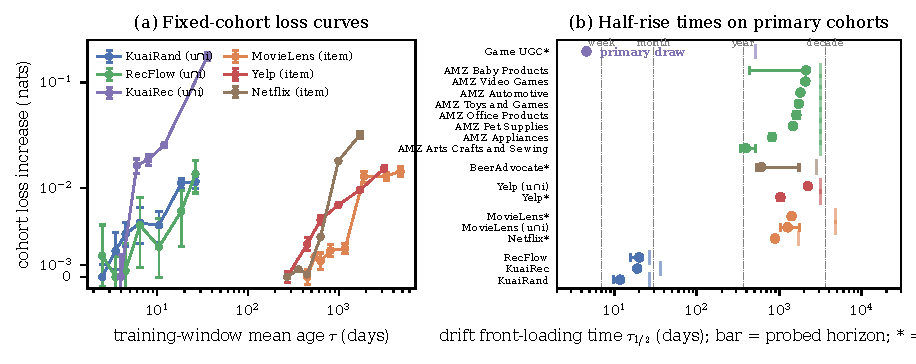
\includegraphics[width=\textwidth]{figs/fig3_spectrum.pdf}
\caption{(a)~Composition-fixed loss curves (cohort loss increase over
the freshest window) for six signal-bearing domains; production logs use the
user${\cap}$item cohort, whereas review platforms use the item cohort
throughout. A symlog loss axis is used because KuaiRec's drift is an order of
magnitude larger than the rest. (b)~Model-free $\tau_{1/2}$ with 90\% bootstrap
CIs, one row per cohort curve. $\tau_{1/2}$ separates into ``weeks'' (feeds) and
``years'' (review corpora), but the vertical bars mark each domain's probing
horizon, which bounds $\tau_{1/2}$ by construction: the apparent clustering
tracks the horizons. The annotated game-UGC point is the original draw;
the cap-by-cap comparison above shows how the second draw changes the result.}
\label{fig:collapse}
\end{figure}

% ===========================================================================
\section{The two blind rounds}
\label{sup:blind}

\subsection{Registration protocol and three caveats}

Round~1 registered the linear dictionary $\hat\delta = a + b\,\ecov$ and its
success criteria before any training run on the held-out categories.
Round~2 registered a mechanistic two-term simulator, revised twice strictly
before unblinding, with each revision archived and validated by retrodiction
on already-measured domains.

Three caveats qualify these claims:

\begin{enumerate}
\item The SHA-256 digests in the code README identify the exact registration
      files shipped in the artifact; their pre-unblinding chronology comes from
      our internal archive rather than an independent external timestamp.
\item The registered success criterion was disjunctive (prediction inside
      the measured 90\% CI \emph{or} absolute error $< 0.35$), whereas
      Table~5 of the main paper scores strictly on the $\pm 0.35$ tolerance.
      Because bound-pinned fits have zero-width CIs, both criteria yield
      identical verdicts across all held-out domains.
\item The constant $\hat\delta \equiv -1$ baseline in Table~5
      was \emph{not} pre-registered; we added it after unblinding to test
      how much of the simulator's apparent accuracy stems from the $[-1, 4]$
      parameter bounds alone, which turn out to account for most of it.
\end{enumerate}

\subsection{Round one: the coverage-elasticity dictionary}

The single training-free statistic is the coverage elasticity
$\ecov = \mathrm{d}\ln \omega / \mathrm{d}\ln\tau$, estimated as the
least-squares slope of $\ln \omega$ on $\ln\tau$ over the translated-arm ages
with $\omega > 10^{-4}$. Across the seven domains available when the dictionary
was constructed, Spearman correlation with $\delta$ was $+0.96$; fitting the
linear rule to the six interior (non-bound) domains yielded a correlation of
$1.00$ and generated the Round-1 predictions.

That correlation decayed monotonically as additional domains entered the panel:
$1.00 \to 0.77 \to 0.57$, settling at $+0.41$ ($p = 0.09$) across the final
19-domain panel ($+0.53$, $p = 0.05$, across the $n = 14$ interior fits:
suggestive, but far short of a predictive dictionary). All three registered
point predictions missed (absolute errors $0.56$, $0.69$, and $1.12$), and all
three erred in the same direction (Figure~\ref{fig:dictionary}a), pointing to an
omitted mechanism rather than random noise. Other intuitive log statistics
(popularity-churn rate, new-item share, and median item age) correlate weakly at
$|\rho| \le 0.19$ ($p \ge 0.45$, $n = 18$--$19$).

\subsection{Round two: the mechanistic simulator}

The round-two predictor needs no training run on the domain it predicts:

\begin{enumerate}
\item measure the held-out domain's coverage curves
      $\omega_A(\tau)$ and $\omega_B(\tau)$ by counting
      (Figure~\ref{fig:dictionary}b);
\item plug in a warm-slope / cold-gap / cold-slope triplet calibrated on
      already-measured domains;
\item simulate the mixture through Eq.~\eqref{eq:twoterm};
\item fit Eq.~\eqref{eq:boxcox} to the simulated curves and report the
      resulting $\delta$.
\end{enumerate}

Only evaluation on the target domain is training-free: the three slope
parameters are estimated from trained probes on eight measured Amazon
categories, and all four hold-outs are likewise Amazon categories. Round~2
therefore tests within-platform transfer from measured to unmeasured
categories.

\subsection{Leave-one-platform-out retrodiction}

Table~\ref{tab:xplat} recalibrates the slope triplets on the measured
domains of every platform \emph{other} than the target's, gives the
simulator nothing but the target's training-free coverage curves, and scores
it against the 14 interior measured exponents. This exercise is a retrodiction
rather than a blind test (the target domains were already measured before the
simulator was designed, with only the calibration split held out) and thus
cannot establish out-of-sample predictive validity. The code path is the
registered one: rebuilding the round-two calibration set reproduces all four
registered predictions to four decimals, so nothing here is an artifact of
re-implementation.

\begin{table}[t]
\centering
\caption{Leave-one-platform-out retrodiction scoring the round-two simulator
(with slope triplets recalibrated on measured domains from all platforms except
the target's) against the 14 interior measured exponents. The last two rows split
those targets by the sign of the measured exponent. A hit is an error within
the same $0.35$ tolerance as Table~5 of the main paper. This is not a blind
test.}
\label{tab:xplat}
\small
\begin{tabular}{lrrr}
\toprule
Predictor / target group & hits & MAE & median AE \\
\midrule
Mechanistic simulator & 2/14 & 1.12 & 0.95 \\
Single statistic ($\ecov$), refit per fold & 3/14 & 0.87 & 0.84 \\
Constant (calibration-set mean) & 2/14 & 1.04 & 1.00 \\
\midrule
\quad simulator, targets with $\delta \le 0$ & 2/5 & 0.28 & --- \\
\quad simulator, targets with $\delta > 0$ & 0/9 & 1.59 & --- \\
\bottomrule
\end{tabular}
\end{table}

Recalibrating \emph{inside} the target's own platform, wherever that
platform has more than one measured domain, gives an MAE of $0.81$ on those
nine targets against $0.96$ across platforms, so most of the error already
arises within a single platform: cross-platform transfer is not the primary
source of failure.

\paragraph{Synthetic coverage sweep.}
For the profiles and parameters tested, flat coverage returns $\delta=0.000$
and the decaying profiles give nonpositive fitted exponents. This is an
empirical property of the tested simulator settings. The cross-platform predictions
span $[-1.00,-0.09]$ while the measurements they target span
$[-0.86, +2.20]$, and their rank correlation with the observed exponents is
$-0.09$ ($p = 0.76$). Three of the four registered round-two predictions were in
fact exactly $-1.0000$, the lower boundary.

\begin{figure}[t]
\centering
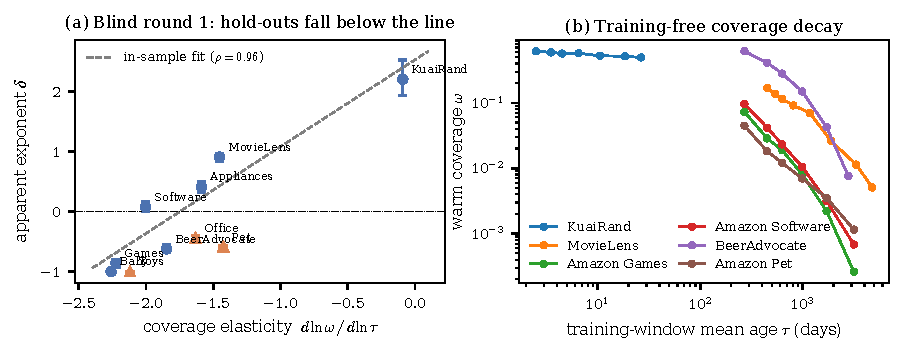
\includegraphics[width=\textwidth]{figs/fig1_mechanism.pdf}
\caption{(a)~Apparent drift exponent $\delta$ (Box--Cox, 90\% bootstrap CIs)
versus coverage elasticity $\ecov$. Round-one hold-outs (triangles) fall
systematically below the in-sample line (dashed), falsifying the
single-statistic dictionary; red points are flagged ``no measurable drift''
and take part in neither the fit nor any correlation. (b)~Training-free
coverage decay curves underlying the mechanistic predictor.}
\label{fig:dictionary}
\end{figure}

% ===========================================================================
\section{Invariance checks and controls}
\label{sup:invariance}

\paragraph{Probe capacity.}
Sweeping capacity over $16\times$ ($d \in \{8, 32, 64, 128\}$) leaves
$\tau_{1/2}$ within the resampling noise of the estimator itself on all
three domains tested (Table~\ref{tab:invariance}). Only the $d = 32$ curves
carry nine seeds, and subsampling the nine-seed KuaiRand cohort down to three
seeds places $\tau_{1/2}$ anywhere in $[4.3, 13.4]$\,d on the exact same
training data (exhaustively across all $\binom{9}{3}$ three-seed subsets). That
reference range is measured on KuaiRand only; on RecFlow the sweep moves
$\tau_{1/2}$ over $20.0$--$22.5$\,d and on MovieLens over $908$--$1{,}263$\,d,
comparable relative movements against which we have no equally exhaustive noise
reference. The sweep therefore supports only the negative statement the
protocol needs: no capacity choice moves $\tau_{1/2}$ by the orders of
magnitude that separate content types. By contrast, the Hill parameter $\Tdrift$
across the same four KuaiRand curves spans $10$--$2{,}650$\,d, which is why we
omit it.

Fitted exponents are far more sensitive to capacity. Cohort $\delta$ on KuaiRand
moves over $0.05$--$0.57$ across the same sweep, RecFlow from $2.42$ up to the
$\delta = 4$ bound, and apparent $\delta$ on KuaiRand over $2.02$--$2.75$
(a range of $0.73$, against the mean bootstrap width of $0.80$ quoted in the
paper). Regime membership is preserved, but point values of $\delta$ are not
probe-invariant, and $\beta$ varies severalfold.

\paragraph{Probe family.}
Replacing the biased-MF probe with a two-tower MLP leaves production-log
apparent exponents essentially unchanged (KuaiRand $2.20 \to 2.22$; RecFlow
$1.70 \to 1.59$) and shifts weak-signal domains within their regime
(MovieLens $0.90 \to 0.61$). The MLP diverged at the default learning rate
on one Amazon category and was retuned there only.

\paragraph{Weekday control.}
Day-of-week periodicity is a plausible confound for a two-week timescale, since
aging 2-day windows fall on different weekday pairs. Rerunning the feed logs
with 7-day windows (which balance all seven weekdays by construction while
holding subsample size $D$ fixed) rules this out, leaving drift intact. The
resulting $\tau_{1/2}$ estimates shift in opposite directions (up on KuaiRand,
down on RecFlow), and both shifts lie within the horizon sensitivity documented
in \S\ref{sup:cohorts}; run at 3 seeds over a shorter age range, the control
excludes the weekday explanation without tightening the estimate. Widening
windows from 2 to 7 days also alters which test events satisfy the every-window
intersection, so this control jointly varies weekday balance and cohort
membership.

\begin{table}[t]
\centering
\caption{$\tau_{1/2}$ (days) under the probe-capacity sweep and the
$W = 7$\,d weekday control (ages $5$--$18$\,d); three seeds per cell except
$d = 32$ (nine; CIs in the paper's Table~6).}
\label{tab:invariance}
\small
\begin{tabular}{lrrrrr}
\toprule
& \multicolumn{4}{c}{probe capacity $d$} & weekday \\
\cmidrule(lr){2-5}
Cohort curve & 8 & 32 & 64 & 128 & control \\
\midrule
KuaiRand (u${\cap}$i) & 11.8 & 11.7 & 8.6 & 12.4 & 14.4 [5.8, 15.3] \\
RecFlow (u${\cap}$i) & 22.5 & 20.0 & 20.9 & 21.2 & 9.9 [8.7, 10.9] \\
MovieLens (u${\cap}$i) & --- & 1{,}263 & 908 & --- & --- \\
\bottomrule
\end{tabular}
\end{table}

\paragraph{Static side-feature two-tower control (\texttt{SideFeatMF}).}
To test whether static user and item metadata eliminates cold-driven aging,
we executed 114 control runs across KuaiRand (36), RecFlow (36), and MovieLens-25M
(42) using identical windows, subsample seeds, and optimization budgets
($d = 32$, $8{,}000$ steps, learning rate $3 \times 10^{-3}$), matching ID-level
subset coverage $\omega_g$ identically against the four-way ID-only MF sweep in
\S\ref{sup:derivations} (max $|\Delta\omega_g| = 0.00$).
\texttt{SideFeatMF} adds learned $d$-dimensional metadata embeddings and scalar
metadata biases to the base MF user and item representations:
\begin{sloppypar}
\begin{itemize}
\item \emph{KuaiRand-Pure} ($1{,}436{,}609$ events, $27{,}077$ users, $7{,}551$
      items): 26 discrete user features (\path{user_active_degree},
      \path{is_lowactive_period}, \path{is_live_streamer},
      \path{is_video_author}, 4 count-range buckets, \path{onehot_feat0..17})
      via \texttt{nn.EmbeddingBag}, plus sparse \path{author_id} (vocabulary
      size $6{,}490$) and 5 discrete item features (\path{video_type},
      \path{upload_type}, \path{music_type}, \path{tag},
      \path{duration_bucket}).
\item \emph{RecFlow} ($30{,}259{,}314$ events across 29 feather shards,
      $36{,}729$ users, $7{,}157{,}647$ items; malformed shard
      \path{2024-02-11.feather} skipped identically to the base log): 3 user
      features (\path{age}, \path{gender}, \path{province}) plus sparse
      \path{author_id} (vocabulary size $2{,}277{,}470$) and 4 discrete item
      features (\path{category_level_one}, \path{category_level_two},
      \path{upload_type}, \path{duration_bucket}).
\item \emph{MovieLens-25M} ($25{,}000{,}095$ events, $162{,}541$ users,
      $59{,}047$ items): 19-dimensional binary movie genre vector ($4{,}568$
      no-genre items).
\end{itemize}
\end{sloppypar}

Table~\ref{tab:sidefeat_full} reports four-way AUCs, joint A${+}$B Box--Cox
exponents across all subsets, and Arm-A two-way cold shares. Adding static
metadata raises $\mathrm{AUC}_{00}$ from ${\approx}0.50$ to $0.54$--$0.64$
and substantially flattens overall $\hat\delta$, yet cold traffic
($\mathbf{10}, \mathbf{01}, \mathbf{00}$) still carries $47.3\%$ (KuaiRand),
$116.9\%$ (RecFlow), and $53.7\%$ (MovieLens-25M) of Arm-A loss aging.

{\sloppy
\paragraph{MovieLens-25M step-200 recalibration note.}
On several younger MovieLens-25M windows, \texttt{SideFeatMF} reaches its best
test loss at the initial checkpoint (step $200$ of $8{,}000$). At that early
checkpoint, unconverged genre and bias scales cause the scalar logit offset
$\Delta\mu$ (fitted on the fresh boundary slice) to overcorrect raw test logits,
inflating recalibrated loss at younger ages and driving the wider-bounds
Box--Cox fit to $\hat\delta = -2.97$ (Table~\ref{tab:sidefeat_full}). Raw loss
($R^2 = 0.961$, $\hat\delta = -0.06$) and calibration-invariant AUC remain well
behaved.\par}

\begin{table}[t]
\centering
\caption{Full \texttt{MF} vs.\ \texttt{SideFeatMF} comparison across KuaiRand,
RecFlow, and MovieLens-25M (114 control runs). Top block reports Arm-A
freshest/oldest AUCs by four-way subset; bottom block gives joint A${+}$B
Box--Cox $\hat\delta$ (in $[-6,4]$ for conditional/recal.\ fits where needed)
and Arm-A cold share $s_{\mathrm{cold}}$.}
\label{tab:sidefeat_full}
\scriptsize
\setlength{\tabcolsep}{2.4pt}
\begin{tabular}{llrrrrrr}
\toprule
Domain & Probe & AUC (fr.) & $\mathrm{AUC}_{11/10/01/00}$ (fr.) & AUC (old) & $\mathrm{AUC}_{11/10/01/00}$ (old) & $\hat\delta_{\mathrm{tot}}$ [90\% CI] & $s_{\mathrm{cold}}$ \\
\midrule
KuaiRand & MF & 0.621 & .614/.625/.648/.503 & 0.593 & .593/.607/.601/.491 & $+$2.14 [+1.89, +2.45] & 50.5\% \\
KuaiRand & SF & 0.652 & .656/.645/.654/.622 & 0.612 & .621/.614/.611/.541 & $+$1.73 [+1.45, +2.07] & 47.3\% \\
RecFlow  & MF & 0.614 & .606/.622/.621/.500 & 0.588 & .597/.606/.608/.500 & $+$1.78 [+1.71, +1.84] & 129.1\% \\
RecFlow  & SF & 0.661 & .665/.662/.655/.635 & 0.645 & .667/.650/.647/.622 & $+$0.41 [+0.24, +0.57] & 116.9\% \\
ML-25M   & MF & 0.703 & .722/.761/.691/.496 & 0.624 & .658/.650/.686/.499 & $+$0.92 [+0.84, +0.98] & 77.5\% \\
ML-25M   & SF & 0.684 & .743/.763/.662/.511 & 0.634 & .656/.633/.689/.544 & $-$0.06 [$-$0.16, +0.06] & 53.7\% \\
\midrule
\multicolumn{8}{c}{\emph{Conditional A${+}$B $\hat\delta$ ($\mathbf{11}$ / $\mathbf{10}$ / $\mathbf{01}$ / $\mathbf{00}$ / recal.)}} \\
\multicolumn{2}{l}{KuaiRand MF / SF} & \multicolumn{6}{l}{MF: $+$4.00 / $+$4.00 / $+$1.36 / $+$0.21 / $+$4.00 \quad|\quad SF: $+$2.49 / $-$0.78 / $+$1.45 / $-$0.01 / $+$1.04} \\
\multicolumn{2}{l}{RecFlow MF / SF}  & \multicolumn{6}{l}{MF: $+$4.00 / $+$1.05 / $+$1.15 / $+$1.17 / $-$0.52 \quad|\quad SF: $+$4.00 / $-$0.08 / $-$6.00 / $+$0.53 / $-$1.23} \\
\multicolumn{2}{l}{ML-25M MF / SF}   & \multicolumn{6}{l}{MF: $-$0.62 / $+$0.13 / $+$3.38 / $-$1.30 / $+$0.39 \quad|\quad SF: $+$1.05 / $+$0.51 / $-$5.52 / $-$6.00 / $-$2.97} \\
\bottomrule
\end{tabular}
\end{table}

% ===========================================================================
\section{The retraining backtest and its policy variants}
\label{sup:backtest}

\paragraph{Setup.}
The backtest slides a $W = 2$\,d training window over a 22-day serving
horizon on RecFlow at six retraining periods,
$P \in \{1, 2, 4, 8, 11, 22\}$ days, for 90 fixed-budget model evaluations
in total (44 at $P = 1$ down to 2 at $P = 22$) at two model seeds. Losses
and AUC are volume-weighted over serving slices. Every volume-weighted
aggregate, across every policy variant run, has a two-seed spread of at most
$0.4$\,mnat and $0.15$ AUC points. Cadence effects exceed that two-seed spread
by an order of magnitude or more; where policy differences in the half-life
sweep below approach this noise floor, we benchmark them explicitly against it.
AUC is computed from a plain rank sum without a tie correction, which is
immaterial at these logit resolutions but is not the textbook estimator. The
static test period is the log's last three days, which the backtest also
serves, so three of the 22 serving days overlap.

On KuaiRec the backtest skips intervals with insufficient training or
serving events. The retained traffic per model seed falls from 10.02M
events at a one-day period to 2.66M at eight days and 1.62M at 16 days.
The observed volume-weighted losses are $0.5287$, $0.5298$, and $0.5350$ nats
at those periods. Because the evaluated events change with cadence, these
aggregates cannot validate a cross-domain optimum on common traffic.

\paragraph{Volume-matching audit.}
The backtest was originally run at $D = 217{,}575$ training events against
the static sweep's $300{,}000$, a $27\%$ mismatch, so the two sides of the
comparison were not volume-matched. Sample size matters at this resolution: in
\S\ref{sup:valstop}, reducing training volume by just $10\%$ shifts $\hat\delta$
by $+0.144$ on RecFlow and $+0.075$ on KuaiRand. We therefore reran the entire
RecFlow backtest at $D = 300{,}000$.

Raising backtest volume from $D = 217{,}575$ to $300{,}000$ halves the
serving-versus-static level offset ($+3.2\text{--}4.3 \to +1.2\text{--}2.6$\,mnat)
and shifts the loss slope ratio from $1.07$ to $1.22$, showing that the static
curve underpredicts the rolling loss slope by ${\sim}18\%$ at matched volume.
Closed-form pricing against interpolated optima remains $1.1$--$2.3\times$
either way, and the ranking-metric loss is unchanged ($-1.85$ vs.\ $-1.86$\,AUC
points). The static-curve comparison and the paper's Table~8 use the
volume-matched runs; the three-way policy comparison uses the original-volume
runs, where all three policies were actually run, against a from-scratch
reference of $0.64878$ nats and $0.6162$ AUC at daily cadence.

The offset is near-constant, not constant: it varies by $1.4$\,mnat across
cadences, a third of the $4.2$\,mnat the serving loss moves across the whole
range, bounding the residual error of cadence comparisons rather than canceling
out.

\paragraph{Stopping rule inside the backtest.}
In the backtest the early-stopping checkpoint is chosen on the very events
the model is serving, and the number of models sharing a serving slice
changes with $P$ (22 models each selecting on about a day at $P = 1$, one
model on 22 days at $P = 22$). If that optimism grew at shorter $P$, it would
artificially inflate measured staleness. Rerunning with the stopping step
chosen on a held-out $10\%$ of each training subsample gives an optimism of
$0.65$--$0.90$\,mnat with no trend in $P$, no larger at $P = 1$ ($0.72$) than
at $P = 22$ ($0.65$). The volume-weighted serving loss rises by $3.54$\,mnat
across the cadence range under the held-out rule against $3.61$ under the
released one (this pair is run at the original $D = 217{,}575$, so it is a
like-for-like test of the stopping rule, not of the volume). The empirical
optimum moves by at most one grid step, at the cheapest of the three prices
only, and the ranking metric falls by a similar amount under both rules ($1.76$
AUC points over the $22\times$ range under the held-out rule, against $1.86$
under the released one).

\paragraph{An asymmetry between the policies.}
Because the from-scratch budget evaluates $160$ candidate checkpoints per run
versus $20$ for warm-starting---and taking the minimum over more draws yields a
stronger downward bias---test-set checkpointing favors the from-scratch policy.
Rerunning all policies under held-out validation stopping removes this
selection bias. The gap narrows as expected without reversing: the warm-start
loss penalty drops from $3.5$--$8.2$\,mnat to $2.6$--$6.4$\,mnat, yet
retraining from scratch still achieves lower loss at every cadence against both
alternatives ($0$ of $6$ reversals each), and warm-starting's daily-cadence AUC
advantage survives at $+0.37$ points against $+0.43$. The one margin that thins
materially is recency's, from $0.9$--$1.6$\,mnat to $0.0$--$0.7$, with the two
policies tied at $P = 11$.

\paragraph{Policy configurations.}
All three policies share the same serving schedule, training windows, and
subsample size $D$. The optimization budget is \emph{not} identical:

\begin{itemize}
\item \emph{From scratch}: $8{,}000$ steps at lr $3\times10^{-3}$, random
      init at every retrain.
\item \emph{Recency}: same budget, but trained on a $4\times$ longer window
      with sample weights halving every half-life. The half-life was
      originally fixed at the window length and never tuned; the sweep below
      varies it.
\item \emph{Warm start}: initializes each retrain from the preceding model
      checkpoint. Because it diverges under the from-scratch budget (see tuning
      notes below), it uses $1{,}000$ steps at learning rate $10^{-4}$.
\end{itemize}

\paragraph{Warm-start hyperparameter sweep.}
Resetting Adam state at the from-scratch budget ($8{,}000$ steps, lr
$3{\times}10^{-3}$) diverges on warm-started weights (serving loss $0.847$,
above $\ln 2$), and lr $10^{-3}$ at $1{,}000$ steps degrades to $0.682$; lr
$10^{-4}$ at $1{,}000$ steps trains stably ($0.657$ vs.\ $0.652$ cold start;
all three configurations are included in the released records). The records also
suggest the budget binds: $62$ of the $78$ warm-started runs select their final
checkpoint ($1{,}000$ steps), i.e., loss is still falling when the budget
expires. By contrast, every $8{,}000$-step run with logged trajectories on this
corpus (both the static sweep and the recency policy) reaches minimum loss near
step $300$ before overfitting. The loss comparison therefore shows that
retraining from scratch wins across each policy's best feasible configuration,
rather than establishing an intrinsic limitation of warm-starting.

\paragraph{Recency half-life sweep.}
Sweeping the half-life over $\{1, 2, 4, 8\}$ days leaves the loss ordering
untouched: the from-scratch policy achieves lower loss at every half-life and
cadence. On AUC, however, the ranking reverses at longer cadences, with AUC
rising monotonically as the half-life lengthens. The 8-day half-life gains
$+0.12$, $+0.16$, $+0.26$, and $+0.37$ AUC points over from-scratch retraining
at $P = 4, 8, 11, 22$\,d while still trailing at 1- and 2-day cadences; the
four-day arm gains $+0.01$, $+0.06$, $+0.17$, and $+0.27$ over the same
cadences.

Against the two-seed spread ($0.4$\,mnat and $0.15$\,AUC points), AUC gains
exceed seed noise at $P \ge 8$ for the eight-day arm and $P \ge 11$ for the
four-day arm, whereas $P = 4$ AUC differences ($+0.12$ and $+0.01$\,points)
and $P \ge 4$ log-loss differences ($0.13$--$0.30$\,mnat) fall within seed
noise. The direction of the reversal is nonetheless the one the flatter
staleness slope predicted ($1.39$ against $1.86$ AUC points lost over the
$22\times$ range). The sweep does not bracket an interior optimum, as AUC
continues to rise at an 8-day half-life.

\paragraph{A protocol precondition.}
Rolling backtests require a calendar-contiguous log. On KuaiRec, 23
sparse or hollow days and a mid-log collection-regime shift change the evaluated
traffic across cadences, precluding like-for-like cross-cadence comparisons.

\paragraph{Strictly non-overlapping multi-domain and dual-metric backtests.}
To eliminate the 3-day overlap between RecFlow's static test window and 22-day
serving horizon---and to evaluate both log loss and ranking ($1{-}\mathrm{AUC}$)
across independent platforms---we ran 296 strictly non-overlapping rolling
backtest runs ($W = 2$\,d, fixed per-domain $D$,
$\max t_{\mathrm{serve}} \le t_{\mathrm{static},0}$ verified for every run, and
identical served-event totals across all periods and seeds;
Table~\ref{tab:backtest_summary_s9}). The three series cover RecFlow ($19$\,d
horizon, $80$ runs, $P \in \{1,2,4,8,11,19\}$\,d), KuaiRand ($22$\,d, $90$
runs, $P \in \{1,2,4,8,11,22\}$\,d), and Game-UGC finish ($32$\,d, $126$ runs,
$P \in \{1,2,4,8,16,32\}$\,d).

Table~\ref{tab:pstar_auc_s9} compares $P^\ast$ pricing under $a{=}0$ versus
$a{=}W/2{=}1$\,d on both Box--Cox and power-form static A-arm curves for
$1{-}\mathrm{AUC}$ (plus log-loss reference). Three structural behaviors emerge:
(i)~on Game-UGC loss, where Box--Cox $\hat\delta{=}-1.657 \le -1$, $a{=}0$ is
undefined whereas $a{=}W/2$ remains finite ($0.13$--$0.54$\,d); (ii)~near
$\delta_{\mathrm{AUC}} \le 0$ (RecFlow $\hat\delta{=}-0.088$, Game-UGC
$\hat\delta{=}-0.494$), $a{=}0$ collapses toward zero ($0.05$--$0.64$\,d on
RecFlow 19\,d, $\le 0.38$\,d on Game-UGC), while $a{=}W/2$ aligns closely with
the tested and interpolated $1{-}\mathrm{AUC}$ optima; and (iii)~on KuaiRand
($\hat\delta{=}2.49$ loss, $4.00$ $1{-}\mathrm{AUC}$), steep static curvature
overpredicts local optima at lower retraining prices.

\begin{table}[t]
\centering
\caption{Summary of all four rolling-retrain backtest series (volume-matched
$D$; 296 strict zero-overlap runs plus the 22-day RecFlow series). ``SR'' is
measured/predicted slope ratio; $r_{\mathrm{age}}$, $r_{\log P}$, and
$r_{\mathrm{lin}}$ are shape correlations against the static age law and two nulls.}
\label{tab:backtest_summary_s9}
\scriptsize
\setlength{\tabcolsep}{3.5pt}
\begin{tabular}{llrrrrrrr}
\toprule
Series (zero ov.) & Metric & Penalty & Pred. & SR & $r_{\mathrm{age}}$ & $r_{\log P}$ & $r_{\mathrm{lin}}$ & 2-seed max \\
\midrule
RecFlow 22\,d (no)   & Loss (mnat)     &  4.17 &  2.83 & 1.220 & 0.988 & 0.977 & 0.987 & 0.16\,m \\
RecFlow 22\,d (no)   & $1{-}\mathrm{AUC}$ & 18.53 & 15.97 & 1.010 & 0.994 & 0.993 & 0.965 & 1.20\,m \\
RecFlow 19\,d (yes)  & Loss (mnat)     &  3.83 &  2.41 & 1.351 & 0.992 & 0.976 & 0.991 & 0.16\,m \\
RecFlow 19\,d (yes)  & $1{-}\mathrm{AUC}$ & 17.08 & 14.64 & 1.005 & 0.995 & 0.992 & 0.979 & 0.96\,m \\
KuaiRand 22\,d (yes) & Loss (mnat)     &  3.72 &  2.15 & 1.153 & 0.855 & 0.850 & 0.775 & 0.29\,m \\
KuaiRand 22\,d (yes) & $1{-}\mathrm{AUC}$ &  9.92 &  5.82 & 1.390 & 0.949 & 0.946 & 0.939 & 1.51\,m \\
Game-UGC 32\,d (yes) & Loss (mnat)     & 15.81 & 13.23 & 0.929 & 0.996 & 0.951 & 0.789 & 2.47\,m \\
Game-UGC 32\,d (yes) & $1{-}\mathrm{AUC}$ & 72.35 & 54.10 & 1.073 & 0.991 & 0.952 & 0.802 & 20.71\,m \\
\bottomrule
\end{tabular}
\end{table}

\begin{table}[t]
\centering
\caption{Cadence pricing $P^\ast$ (days) for $1{-}\mathrm{AUC}$ across the
three strictly non-overlapping backtests (plus Game-UGC loss where $a{=}0$
diverges), comparing $a{=}0$ vs.\ $a{=}W/2{=}1$\,d under Box--Cox (BC) and
power-form (Pow) static fits against Tested and Interp.\ optima.}
\label{tab:pstar_auc_s9}
\scriptsize
\setlength{\tabcolsep}{3.5pt}
\begin{tabular}{llrrrrrr}
\toprule
Series / metric & $\lambda C$ & BC ($a{=}0$) & Pow ($a{=}0$) & BC ($a{=}W/2$) & Pow ($a{=}W/2$) & Tested & Interp. \\
\midrule
RecFlow 19\,d ($1{-}\mathrm{AUC}$) & $10^{-2.5}$ & 0.18 & 0.28 & 0.86 & 0.95 & 1 & 1.20 \\
RecFlow 19\,d ($1{-}\mathrm{AUC}$) & $10^{-2}$   & 0.64 & 0.89 & 1.81 & 1.97 & 2 & 2.00 \\
RecFlow 19\,d ($1{-}\mathrm{AUC}$) & $10^{-1.5}$ & 2.26 & 2.80 & 4.21 & 4.49 & 8 & 5.62 \\
RecFlow 19\,d ($1{-}\mathrm{AUC}$) & $10^{-1}$   & 7.99 & 8.82 & 11.07 & 11.30 & 11 & 11.33 \\
\midrule
KuaiRand 22\,d ($1{-}\mathrm{AUC}$) & $10^{-3}$  & 7.55 & 7.55 & 6.81 & 6.81 & 1 & 1.00 \\
KuaiRand 22\,d ($1{-}\mathrm{AUC}$) & $10^{-2.5}$ & 9.50 & 9.50 & 8.76 & 8.76 & 2 & 1.64 \\
KuaiRand 22\,d ($1{-}\mathrm{AUC}$) & $10^{-2}$  & 11.96 & 11.96 & 11.22 & 11.22 & 8 & 7.97 \\
KuaiRand 22\,d ($1{-}\mathrm{AUC}$) & $10^{-1}$  & 18.96 & 18.96 & 18.21 & 18.21 & 22 & 22.00 \\
\midrule
Game-UGC 32\,d ($1{-}\mathrm{AUC}$) & $10^{-2}$  & 0.004 & 0.55 & 0.63 & 1.44 & 1 & 1.00 \\
Game-UGC 32\,d ($1{-}\mathrm{AUC}$) & $10^{-1.5}$ & 0.039 & 1.74 & 1.38 & 3.15 & 2 & 2.00 \\
Game-UGC 32\,d ($1{-}\mathrm{AUC}$) & $10^{-1}$  & 0.377 & 5.47 & 3.54 & 7.60 & 4 & 3.98 \\
\midrule
Game-UGC 32\,d (Loss) & $10^{-3}$   & undef. & 0.34 & 0.13 & 1.06 & 1 & 1.00 \\
Game-UGC 32\,d (Loss) & $10^{-2.5}$ & undef. & 1.08 & 0.25 & 2.25 & 1 & 1.00 \\
Game-UGC 32\,d (Loss) & $10^{-2}$   & undef. & 3.40 & 0.54 & 5.21 & 2 & 2.00 \\
\bottomrule
\end{tabular}
\end{table}

% ===========================================================================
\section{Datasets and preprocessing}
\label{sup:data}

\paragraph{Inputs.}
The core protocol requires only four fields per event: user ID, item ID,
timestamp, and binary label. All IDs are integer-encoded; the primary study
uses no raw identifiers, text, or side features (the three-domain static
metadata control is documented separately in \S\ref{sup:invariance}).

\paragraph{Panel.}
The panel is 11 logs from 9 platforms, yielding 23 domains
(log $\times$ label). Three short-video exposure logs (KuaiRand-Pure,
RecFlow realshow, the long-window KuaiRec big matrix) are separate
collections, from different periods and pipelines, of the same short-video
ecosystem, so we count them as one platform. Twelve Amazon categories share
a single platform, user base, rating scale, preprocessing pipeline,
and (most consequentially) ``one-and-done'' reviewer coverage
dynamics; five were used for initial calibration and seven were
held out for the two blind rounds. The 68 measurement settings are 23
apparent-law fits, 33 cohort fits (26 distinct plus 7 capacity-sweep
replicas), 7 apparent capacity replicas, and 5 MLP-probe fits.

\paragraph{Labels.}
Labels are binarized per domain: rating $\ge 4$ on the review corpora,
rating $= 5$ on Epinions, watch-ratio $\ge 1$ on KuaiRec, and click or
effective view on the other feed logs. Base rates differ widely across the
panel ($0.34$--$0.88$). Both label semantics and observation horizon matter
when comparing shapes or timescales across domains (for instance, the play
and finish labels on the game-UGC log yield descending and rising cohort
curves); absolute loss penalties are likewise \emph{not} comparable across
labels, which is why the paper checks its one cross-label comparison (the
drift-rate column) against a scale-free elasticity.

\paragraph{Windows.}
Each domain has one fixed test period, the final 2--6 time units of the log
(days on the feed logs, months elsewhere). Two manipulations are run against
it: (A)~a window of fixed length translated back by log-spaced gaps, and
(B)~windows ending at the test boundary with log-spaced spans. Every window
is uniformly subsampled to the same event count $D$, the minimum surviving
window volume, capped at $300{,}000$. $D$ is held fixed within a domain but
not across domains ($25$K--$300$K), so it covaries with domain identity in
every cross-domain regression. The released code calls the two arms
\texttt{A} and \texttt{C}.

\paragraph{Two corpus-specific caveats.}
The Kaggle Steam release retains only 315 head titles, so its ``no
measurable drift'' verdict is a statement about head games, not about the
platform; at $\omega = 0.004$ essentially every test event is cold. On
Epinions, $94\%$ of events occur in a single 2001 burst, violating
stationary sampling; this domain is reported for completeness and excluded by
our pre-stated quality-control rule.

\paragraph{The industrial game-UGC log.}
This corpus spans 42.8M impressions across 4.48M users and 274K user-created
items (with logged exposure negatives) over 18 months, evaluated under two
binary targets (a play label and a finish/depth label). At 9.6 events per user
it is the panel's only low-recurrence ecosystem: the composition-fixed
\emph{user} cohort is empty even though $50\%$ of users appear in $\ge 2$ time
bins, because sparse returns do not land in the same narrow windows, which is
why item appeal is the right observable. This log was provided under an
agreement that permits aggregate reporting only. We release all derived
per-run measurements (losses and coverage statistics) rather than the raw
interaction log; none of the released aggregates can be inverted to reconstruct
individual behavior.

% ===========================================================================
\section{Code, run records, and reproduction}
\label{sup:code}

All source code, per-run records (JSONL), blind-round registration files,
figure scripts, and per-domain configuration tables are available at:
\begin{center}
\url{https://github.com/minghaochen/data-aging-wsdm27}
\end{center}

\noindent
The repository includes the following analyses.

\begin{sloppypar}
\begin{itemize}
\item \path{src/paper_numbers.py} produces the primary panel summaries and run census.
\item \path{src/age_diagnostics.py} reproduces the adjacent-age decomposition,
      all game-UGC caps and redraws, and the RecFlow log-loss cadence
      comparison in the paper's Table~8.
      It writes \path{results/age_diagnostics.json}.
\item \path{src/cr_lib.py}, \path{src/stage1_zero_run.py}--\path{src/stage5_gameugc_hygiene.py},
      and \path{src/camera_ready_reproduce.py} implement and verify the
      1,385 diagnostic-extension runs and training-free log audits, writing
      \path{results/stage1_zero_run.json} and \path{results/stage2_fourway_summary.json}--\path{results/stage5_gameugc_summary.json}.
\item \path{src/fig_overview.py} builds Figure~1, and \path{src/paper_figs.py}
      regenerates Figures~2--5 and appendix Figures~S1--S2 from the run records.
\item \path{src/fit_domains.py} implements the Box--Cox fit, the flags, and the
      bootstrap described in \S\ref{sup:protocol} (\path{src/fit.py} and
      \path{src/fit_kuairand.py} are legacy exploratory scripts).
\item \path{src/blind_predict.py} and \path{src/blind_predict2.py} are the
      two registered predictors, and \path{src/cross_platform_test.py} the
      leave-one-platform-out retrodiction of \S\ref{sup:blind}.
\item \path{src/backtest.py}, \path{src/backtest_baselines.py},
      \path{src/backtest_analysis.py}, \path{src/backtest_compare.py}, and
      \path{src/recency_halflife_analysis.py} implement
      \S\ref{sup:backtest}.
\item \path{src/valstop_analysis.py} (\S\ref{sup:valstop}) and
      \path{src/policy_valstop_analysis.py} (\S\ref{sup:valstop} and
      \S\ref{sup:backtest}) implement the stopping-rule analyses;
      \path{src/cohort_seed_analysis.py} the cohort realization check of
      \S\ref{sup:cohorts}; and \path{src/period_analysis.py} the sweep of
      \S\ref{sup:periods}.
\end{itemize}
\end{sloppypar}

\begin{sloppypar}
\noindent
Key result files for specific diagnostic and control claims ship directly in \path{results/}:
\begin{itemize}
\item \emph{Backtest volume and policy controls}: \path{results/backtest_recflow__d300k.jsonl} stores the volume-matched ($D = 300{,}000$) backtest underlying Figure~5 and the $1.22$ slope ratio (vs.\ \path{results/backtest_recflow.jsonl} at $D = 217{,}575$); \path{results/backtest_recflow__recency_hl*.jsonl} stores the recency half-life sweep.
\item \emph{Convention, cohort, and retrodiction checks}: \path{results/valstop_analysis.json} and \path{results/policy_valstop.json} store the held-out stopping-rule reruns; \path{results/cohort_seed_sensitivity.json} stores the second feed-cohort draw; \path{results/cross_platform_test.json} stores the leave-one-platform-out folds; and \path{results/age_diagnostics.json} stores the two-way attribution and cadence summaries.
\item \emph{Extended CPU diagnostics ($1{,}385$ runs)}: \path{results/fourway_*.jsonl} (23 files, 522 runs), \path{results/backtest_recflow_nooverlap19d.jsonl} (80 runs), \path{results/backtest_kuairand_strict.jsonl} (90 runs), \path{results/backtest_gameugc_strict.jsonl} (126 runs), \path{results/sidefeat_*.jsonl} (3 files, 114 runs), and \path{results/gameugc_finish__icohort_draws.jsonl}, \path{results/gameugc_finish__valstop.jsonl}, \path{results/gameugc_finish__icohort_valstop.jsonl}, and \path{results/gameugc_finish__icohort_finegrid.jsonl} (453 runs), summarized in \path{results/stage1_zero_run.json} and \path{results/stage2_fourway_summary.json}--\path{results/stage5_gameugc_summary.json}.
\item \emph{Blind registrations}: \path{results/blind_predictions.json} and \path{results/blind_predictions_round2.json} contain the frozen Round-1 and Round-2 predictions recorded prior to training on the respective held-out domains.
\end{itemize}
\end{sloppypar}

Public datasets are used under their published terms and are not
redistributed; the preparation scripts (\path{src/prep_*.py}) take the
official releases as input. Two practical points govern offline reproduction
without raw data. Every analysis in \path{src/paper_numbers.py},
\path{src/age_diagnostics.py}, \path{src/camera_ready_reproduce.py}, and the
\texttt{--summary-only} modes of \path{src/stage2_fourway_cold.py},
\path{src/stage3_backtests.py}, and \path{src/stage5_gameugc_hygiene.py} run
from \path{results/} alone \emph{except}
the age-convention section (\S\ref{sup:agewt}), which has to re-read the
timestamps inside each training window and therefore needs the prepared
datasets in \path{data/}; when \path{data/} is absent, that section logs a
skip notice and all remaining outputs reproduce unchanged. For the same reason
\path{src/cross_platform_test.py} recomputes coverage curves from
\path{data/}, and its published output is shipped as
\path{results/cross_platform_test.json} for readers who do not rebuild the
datasets; similarly, \path{src/stage1_zero_run.py} and
\path{src/stage4_side_features.py} (whose raw feature caches are not
redistributed) ship their verified outputs in \path{results/stage*_*.json}. The industrial
game-UGC log is not released, for the reason given in \S\ref{sup:data}; its
derived per-run measurements are.

A full baseline reproduction is roughly 40 GPU hours on a single NVIDIA
GTX~1660 (6\,GB; any single domain reproduces in about an hour), and the
1,385 extended CPU \texttt{SparseAdam} diagnostic runs completed in under a day.

\end{document}
